\documentclass[a4paper]{book}
\usepackage[margin=1in]{geometry}
\usepackage[T1]{fontenc}
\usepackage[utf8]{inputenc}
\usepackage[hidelinks]{hyperref}
\usepackage{amsmath}
\usepackage{amssymb}
\usepackage{enumerate}
\usepackage{setspace}
\usepackage{listings}
\usepackage{xcolor}
\usepackage{amsthm}
\usepackage{xspace}
\usepackage{adjustbox}
\usepackage{booktabs} 
\usepackage{array}    
\usepackage{adjustbox} 
\usepackage{colortbl}
\usepackage{graphicx}
\usepackage{ocgx2}
\usepackage{lipsum}
\usepackage{tcolorbox}
\usepackage{caption}

% Configuration pour les listings de code
\definecolor{codebg}{RGB}{245,245,245}
\lstset{
    backgroundcolor=\color{codebg},
    basicstyle=\ttfamily\small,
    frame=single,
    breaklines=true,
    columns=fullflexible,
    keywordstyle=\color{blue},
    commentstyle=\color{gray},
    stringstyle=\color{orange},
    showstringspaces=false
}
\setstretch{1.15}

%----- TITLE PAGE INFO -----%
\title{\Huge \textbf{Spanning Tree Protocol (STP) Workbook}\\
       \Large Fundamentals, Variants, Tuning, and Practical Labs}
\author{\Large Written for Networking Students and Professionals}
\date{\today}

\begin{document}

%----- MODERN TITLE PAGE -----%
\begin{titlepage}
<<<<<<< HEAD
    \centering
    \vspace*{4cm}
    {\Huge \textbf{Spanning Tree Protocol (STP) Workbook}\par}
    \vspace{0.8cm}
    {\Large A Hands-On Guide to PVST+, RSTP, and MSTP\par}
    \vspace{0.3cm}
    \rule{0.9\textwidth}{1pt}
    
    \vspace{0.6cm}
    {\large \textbf{Mehdi JAFARI ZADEH}}\par
    \vspace{0.3cm}
=======
	\centering
	\vspace*{4cm}
	{\Huge \textbf{Spanning Tree Protocol (STP) Workbook}\par}
	\vspace{0.8cm}
	{\Large A Hands-On Guide to PVST+, RSTP, and MSTP\par}
	\vspace{0.3cm}
	\rule{0.9\textwidth}{1pt}

	\vspace{0.6cm}
	{\large \textbf{Mehdi JAFARI ZADEH}}\par
	\vspace{0.3cm}
>>>>>>> stp


	\vfill
	\textbf{Date:} \today
	\vspace{2cm}
\end{titlepage}


\tableofcontents
\newpage

%------------------------------------------------------
% Chapter 1: STP Introduction
%------------------------------------------------------
\chapter{Spanning Tree Protocol (STP)}

\section*{STP Introduction}

Spanning Tree Protocol (STP) is essential for preventing broadcast storms and loops in switched networks with redundant paths. In this section, we'll cover the purpose of STP, its importance in maintaining a loop-free topology, and an overview of how it dynamically reconfigures the network when changes occur. This foundation sets the stage for understanding how STP supports network reliability and resilience.

\section*{Root Bridge}
The Root Bridge is the central reference point in the STP topology. It is elected based on the lowest bridge ID, which is a combination of the bridge priority and MAC address. All other switches in the network compute the best path back to the Root Bridge. Understanding how the Root Bridge is selected is crucial because it directly influences the network's spanning tree structure and the flow of data through the network.

\section*{STP Root Port, Designated Port}
Within each switch (except for the Root Bridge), the Root Port is the interface that offers the best path to the Root Bridge, based on the lowest path cost. On each network segment, the Designated Port is the switch port that has the best path to the Root Bridge and is responsible for forwarding traffic toward it. Together, these port roles determine the active topology of the network by ensuring there is only one active path between any two network devices, thereby preventing loops.


\begin{figure}[h]
	\centering
	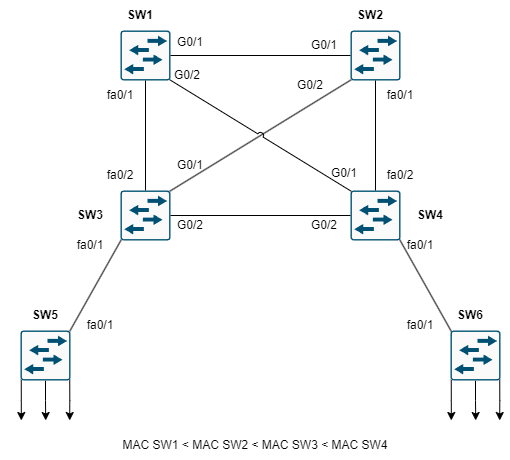
\includegraphics[width=0.9\textwidth]{img/stp01.png}
	\caption{\textit{}}
\end{figure}

\subsection*{Network Topology Overview}
In this exercise, you will work with the network topology as described below. The switches (SW1 to SW6) are connected as Figure 1.1.



The MAC addresses of the switches are as follows:
\begin{center}
	{MAC SW1 $<$ MAC SW2 $<$ MAC SW3 $<$ MAC SW4 $<$ MAC SW6 $<$ MAC SW6}
\end{center}
This means \textbf{SW1} has the lowest MAC address and \textbf{SW6} has the highest.
\newpage
\section*{Step-by-Step Tasks}

\begin{enumerate}
	\item \textbf{Switch STP Mode to Traditional STP} \\
	      Change the STP mode on all switches to \textbf{traditional STP (IEEE 802.1D)}.

	      %==========================
	      \switchocg{codeblock}{%
		      \color{black}\underline{Click here to display the answer:}%
	      }


	      \begin{ocg}{Code Block}{codeblock}{0}
		      \vspace{0.5cm}
		      \begin{lstlisting}
Switch(config)# spanning-tree mode stp
\end{lstlisting}

	      \end{ocg}
	      %=================================

	\item \textbf{Disable Unused Interfaces} \\
	      Turn off any extra or unused interfaces to prevent unnecessary loops.

	      %==========================
	      \switchocg{codeblock}{%
		      \color{black}\underline{Click here to display the answer:}%
	      }


	      \begin{ocg}{Code Block}{codeblock}{0}
		      \vspace{0.5cm}
		      \begin{lstlisting}
Switch(config)# interface [interface-id]
Switch(config)# shutdown

\end{lstlisting}

	      \end{ocg}
	      %=================================


	\item \textbf{Set Links to Point-to-Point Mode} \\
	      Configure all links between switches as \textbf{Point-to-Point (P2P)} to optimize STP convergence.

	      %==========================
	      \switchocg{codeblock}{%
		      \color{black}\underline{Click here to display the answer:}%
	      }


	      \begin{ocg}{Code Block}{codeblock}{0}
		      \vspace{0.5cm}
		      \begin{lstlisting}
Switch(config)# spanning-tree link-type point-to-point


\end{lstlisting}

	      \end{ocg}
	      %=================================

	\item \textbf{Verify Bridge IDs} \\
	      Check the \textbf{Bridge ID} for each switch to see how STP will select the Root Bridge.

	      %==========================
	      \switchocg{codeblock}{%
		      \color{black}\underline{Click here to display the answer:}%
	      }


	      \begin{ocg}{Code Block}{codeblock}{0}
		      \vspace{0.5cm}
		      \begin{lstlisting}
Switch(config)# show spanning-tree
\end{lstlisting}

	      \end{ocg}
	      %=================================

	\item \textbf{Predict the Root Bridge} \\
	      Based on the MAC addresses provided (\textbf{SW1 $<$ SW2 $<$ SW3 $<$ SW4 $<$ SW5 $<$ SW6}), estimate which switch will become the Root Bridge.
	      \begin{itemize}
		      \item \textit{Question:} Which switch is likely to be the Root Bridge and why?
	      \end{itemize}


	      %==========================

	      \switchocg{codeblock}{
		      \color{black}\underline{Click here to display the answer:}%
	      }

	      \begin{ocg}{Code Block}{codeblock}{0}
		      \vspace{0.5cm}
		      \tcbset{colback=gray!10, colframe=gray!50, boxrule=0.5pt, arc=4pt, left=4pt, right=4pt, top=4pt, bottom=4pt}
		      \begin{tcolorbox}
			      \small{
				      The switch with the lowest MAC address will be selected as the Root Bridge. According to the provided MAC address order:

				      MAC SW1 < MAC SW2 < MAC SW3 < MAC SW4

				      Therefore, SW1 will be the Root Bridge.
			      }
		      \end{tcolorbox}
	      \end{ocg}

	      %=================================


	\item \textbf{Estimate Root Ports} \\
	      Identify the \textbf{Root Port} on each non-root switch. This is the port with the lowest path cost to the Root Bridge.
	      \begin{itemize}
		      \item \textit{Question:} Which port will be the Root Port on SW2, SW3, SW4, SW5, and SW6?
	      \end{itemize}

	      %==========================

	      \switchocg{codeblock}{
		      \color{black}\underline{Click here to display the answer:}%
	      }

	      \begin{ocg}{Code Block}{codeblock}{0}
		      \vspace{0.5cm}
		      \tcbset{colback=gray!10, colframe=gray!50, boxrule=0.5pt, arc=4pt, left=4pt, right=4pt, top=4pt, bottom=4pt}
		      \begin{tcolorbox}
			      \small{
				      \begin{itemize}
					      \item \textbf{SW2:}
					            \begin{itemize}
						            \item \textit{G0/1 $\rightarrow$ SW1 (cost = 4)}
					            \end{itemize}

					      \item \textbf{SW3:}
					            \begin{itemize}
						            \item \textit{G0/1 $\rightarrow$ SW2 (cost = 4) + G0/1 $\rightarrow$ SW1 (cost = 4) = 8}
					            \end{itemize}

					      \item \textbf{SW4:}
					            \begin{itemize}
						            \item \textit{G0/1 $\rightarrow$ SW1 (cost = 4)}
					            \end{itemize}

					      \item \textbf{SW5:}
					            \begin{itemize}
						            \item \textit{F0/1 $\rightarrow$ SW3 (cost = 19) + G0/1 $\rightarrow$ SW2 (cost = 4) + G0/1 $\rightarrow$ SW1 (cost = 4) = 27}
					            \end{itemize}

					      \item \textbf{SW6:}
					            \begin{itemize}
						            \item \textit{F0/1 $\rightarrow$ SW4 (cost = 19) + G0/1 $\rightarrow$ SW1 (cost = 4) = 23}
					            \end{itemize}
				      \end{itemize}
			      }
		      \end{tcolorbox}
	      \end{ocg}

	      %=================================

	\item \textbf{How Many Root Bridges Are There in a Network?}
	      \begin{itemize}
		      \item \textit{Question:} In any given STP-enabled network, how many Root Bridges can exist?
	      \end{itemize}
	      %==========================

	      \switchocg{codeblock}{
		      \color{black}\underline{Click here to display the answer:}%
	      }

	      \begin{ocg}{Code Block}{codeblock}{0}
		      \vspace{0.5cm}
		      \tcbset{colback=gray!10, colframe=gray!50, boxrule=0.5pt, arc=4pt, left=4pt, right=4pt, top=4pt, bottom=4pt}
		      \begin{tcolorbox}
			      \small{
				      In any STP-enabled network, there can only be one Root Bridge per VLAN.
			      }
		      \end{tcolorbox}
	      \end{ocg}

	      %=================================


	\item \textbf{How Many Root Ports Are There in a Network?}
	      \begin{itemize}
		      \item \textit{Question:} In any given STP-enabled network, how many Root Port can exist?
	      \end{itemize}
	      %==========================

	      \switchocg{codeblock}{
		      \color{black}\underline{Click here to display the answer:}%
	      }

	      \begin{ocg}{Code Block}{codeblock}{0}
		      \vspace{0.5cm}
		      \tcbset{colback=gray!10, colframe=gray!50, boxrule=0.5pt, arc=4pt, left=4pt, right=4pt, top=4pt, bottom=4pt}
		      \begin{tcolorbox}
			      \small{
				      Each non-root switch will have one Root Port. Since SW1 is the Root Bridge and there are 5 other switches (SW2, SW3, SW4, SW5, SW6), there will be:

				      Total Root Ports = 5
			      }
		      \end{tcolorbox}
	      \end{ocg}

	      %=================================

	\item \textbf{How Many Designated Ports (DP) Are in the Topology?}
	      \begin{itemize}
		      \item \textit{Question:} In any STP-enabled topology, how many Designated Ports (DP) will there be?
	      \end{itemize}

	      %---,,,,,,,,,,,,,,,,,,,,,,,,,,,,,,,,,,---

	      \switchocg{codeblock}{
		      \color{black}\underline{Click here to display the answer:}%
	      }

	      \begin{ocg}{Code Block}{codeblock}{0}
		      \vspace{0.5cm}
		      \tcbset{colback=gray!10, colframe=gray!50, boxrule=0.5pt, arc=4pt, left=4pt, right=4pt, top=4pt, bottom=4pt}
		      \begin{tcolorbox}
			      \small{
				      In any STP-enabled topology, each network segment will have exactly one Designated Port (DP).

				      A network segment is a link between two switches or a switch and an end device.
			      }
		      \end{tcolorbox}
	      \end{ocg}

	      %---''''''''''''''''''''''''''''''''---

	\item \textbf{Estimate the Designated Ports on Each Switch}
	      \begin{itemize}
		      \item Before using any commands, predict which ports will be Designated Ports on each switch in the topology.
	      \end{itemize}

	\item \textbf{Verify Designated Ports Using Commands}
	      %---,,,,,,,,,,,,,,,,,,,,,,,,,,,,,,,,,,---
	      \switchocg{codeblock}{%
		      \color{black}\underline{Click here to display the answer:}%
	      }


	      \begin{ocg}{Code Block}{codeblock}{0}
		      \vspace{0.5cm}
		      \begin{lstlisting}
Switch(config)# show spanning-tree
\end{lstlisting}

	      \end{ocg}
	      %---''''''''''''''''''''''''''''''''---

	\item \textbf{Are All Root Bridge Ports Designated Ports?}
	      \begin{itemize}
		      \item \textit{Question:} Based on your observations, can you conclude that all ports on the Root Bridge are Designated Ports?
	      \end{itemize}
	      %---,,,,,,,,,,,,,,,,,,,,,,,,,,,,,,,,,,---

	      \switchocg{codeblock}{
		      \color{black}\underline{Click here to display the answer:}%
	      }

	      \begin{ocg}{Code Block}{codeblock}{0}
		      \vspace{0.5cm}
		      \tcbset{colback=gray!10, colframe=gray!50, boxrule=0.5pt, arc=4pt, left=4pt, right=4pt, top=4pt, bottom=4pt}
		      \begin{tcolorbox}
			      \small{
				      Yes, all ports on the Root Bridge are Designated Ports (DPs). The Root Bridge does not have any Root Ports because it is the reference point for all path calculations. Since it provides the shortest path to itself, all its ports are designated to forward traffic.
			      }
		      \end{tcolorbox}
	      \end{ocg}

	      %---''''''''''''''''''''''''''''''''---
	\item \textbf{Change the Port Cost of G0/2 on SW4}
	      \begin{itemize}
		      \item Modify the path cost of interface G0/2 on SW4 to 15. This will influence STP’s decision on which path to use.
	      \end{itemize}
	      %---,,,,,,,,,,,,,,,,,,,,,,,,,,,,,,,,,,---
	      \switchocg{codeblock}{%
		      \color{black}\underline{Click here to display the answer:}%
	      }


	      \begin{ocg}{Code Block}{codeblock}{0}
		      \vspace{0.5cm}
		      \begin{lstlisting}
Switch(config)# interface g0/2
Switch(config-if)# spanning-tree cost 15

\end{lstlisting}

	      \end{ocg}
	      %---''''''''''''''''''''''''''''''''---
	      \begin{figure}[h]
		      \centering
		      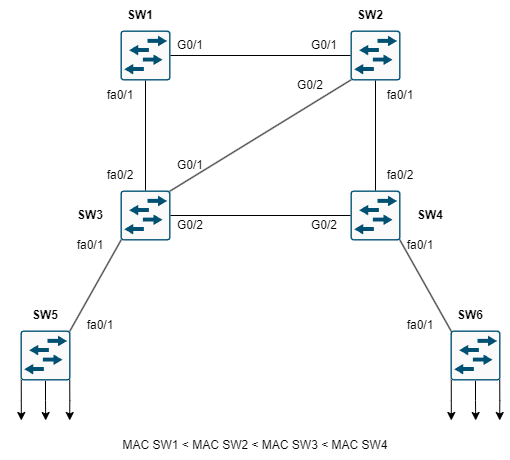
\includegraphics[width=0.9\textwidth]{img/stp02.png}
		      \caption{\textit{}}
	      \end{figure}
	      \newpage


	\item \textbf{Predict the New Root Port on SW4 After Link Removal}
	      \begin{itemize}
		      \item If you remove the link connected to G0/1 on SW4 (Figure 1.2), which port will become the new Root Port? Explain your reasoning based on path costs and STP rules.
		      \item \textit{Hint:} Consider which remaining port on SW4 has the lowest cost path to the Root Bridge.

		            %---,,,,,,,,,,,,,,,,,,,,,,,,,,,,,,,,,,---

		            \switchocg{codeblock}{
			            \color{black}\underline{Click here to display the answer:}%
		            }

		            \begin{ocg}{Code Block}{codeblock}{0}
			            \vspace{0.5cm}
			            \tcbset{colback=gray!10, colframe=gray!50, boxrule=0.5pt, arc=4pt, left=4pt, right=4pt, top=4pt, bottom=4pt}
			            \begin{tcolorbox}
				            \small{


					            \begin{itemize}
						            \item \textit{F0/2 $\rightarrow$ SW2 (cost = 19) + G0/1 $\rightarrow$ SW1 (cost = 4) = 23}
						            \item \textit{G0/2 $\rightarrow$ SW3 (cost = 15) + G0/1 $\rightarrow$ SW2 (cost = 4) + G0/1 $\rightarrow$ SW1 (cost = 4)= 23}
					            \end{itemize}
					            In cases where the interface costs are equal, a tiebreaker is required. In such situations, the path with the lower Bridge ID (BID) of the sending switch is selected.

					            Since the MAC address of Switch 2 is lower than that of Switch 3, the interface Fa0/1 is selected.
				            }
			            \end{tcolorbox}
		            \end{ocg}

		            %---''''''''''''''''''''''''''''''''---
	      \end{itemize}


\end{enumerate}

\newpage
\section*{Additional Exercises}

\subsection*{Draw the Active Topology for Each Scenario}

\begin{minipage}{0.4\textwidth}
	\centering
	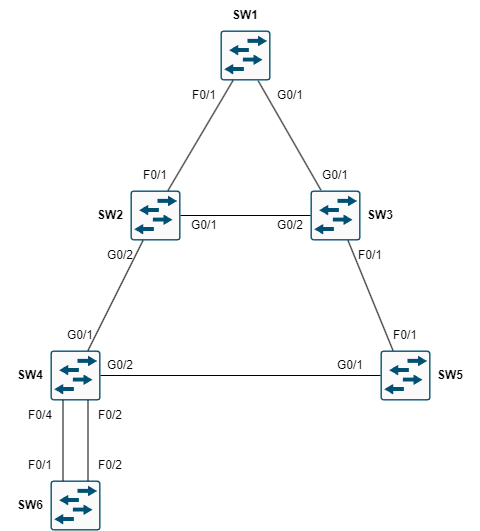
\includegraphics[width=\linewidth]{img/stp03.png}
	\captionof{figure}{\textit{Scenario 1 Topology}}
\end{minipage}%
\hfill
\begin{minipage}{0.55\textwidth}
	\vspace{2cm}
	%---,,,,,,,,,,,,,,,,,,,,,,,,,,,,,,,,,,---

	\switchocg{codeblock}{
		\color{black}\underline{Click here to display the answer:}%
	}

	\begin{ocg}{Code Block}{codeblock}{0}

		\tcbset{colback=gray!10, colframe=gray!50, boxrule=0.5pt, arc=4pt, left=4pt, right=4pt, top=4pt, bottom=4pt}
		\begin{tcolorbox}
			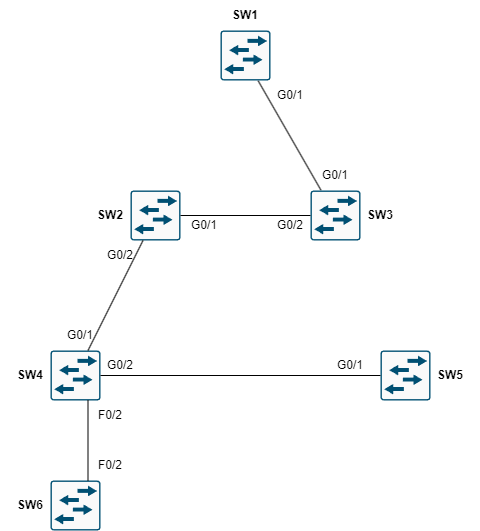
\includegraphics[width=\linewidth]{img/stp03active.png}
		\end{tcolorbox}
	\end{ocg}

	%---''''''''''''''''''''''''''''''''---

\end{minipage}
\vspace{2cm}


\begin{minipage}{0.4\textwidth}
	\centering
	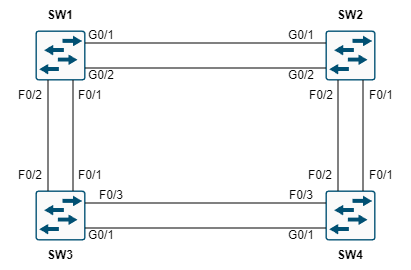
\includegraphics[width=\linewidth]{img/stp04.png}
	\captionof{figure}{\textit{Scenario 2 Topology}}
\end{minipage}%
\hfill
\begin{minipage}{0.55\textwidth}

	%---,,,,,,,,,,,,,,,,,,,,,,,,,,,,,,,,,,---

	\switchocg{codeblock}{
		\color{black}\underline{Click here to display the answer:}%
	}

	\begin{ocg}{Code Block}{codeblock}{0}

		\tcbset{colback=gray!10, colframe=gray!50, boxrule=0.5pt, arc=4pt, left=4pt, right=4pt, top=4pt, bottom=4pt}
		\begin{tcolorbox}

			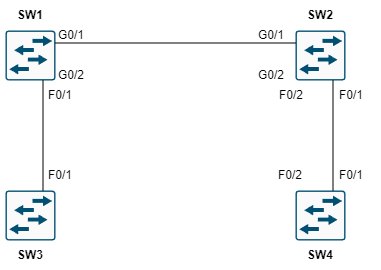
\includegraphics[width=\linewidth]{img/stp04active.png}
		\end{tcolorbox}
	\end{ocg}

	%---''''''''''''''''''''''''''''''''---    
\end{minipage}

\newpage

\centering
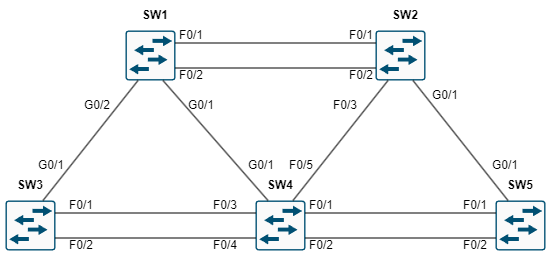
\includegraphics[width=0.7\textwidth]{img/stp05.png}
\captionof{figure}{\textit{Scenario 3 Topology}}
\vspace{2cm}

\begin{minipage}{0.55\textwidth}
	%---,,,,,,,,,,,,,,,,,,,,,,,,,,,,,,,,,,---

	\switchocg{codeblock}{
		\color{black}\underline{Click here to display the answer:}%
	}

	\begin{ocg}{Code Block}{codeblock}{0}

		\tcbset{colback=gray!10, colframe=gray!50, boxrule=0.5pt, arc=4pt, left=4pt, right=4pt, top=4pt, bottom=4pt}
		\begin{tcolorbox}

			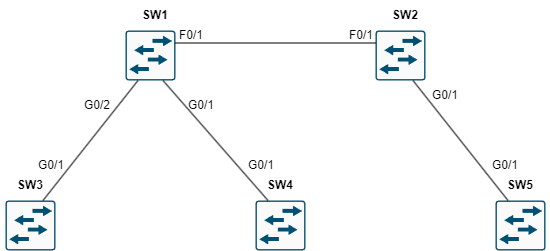
\includegraphics[width=1\textwidth]{img/stp05active.png}
		\end{tcolorbox}
	\end{ocg}

	%---''''''''''''''''''''''''''''''''---   
\end{minipage}


%------------------------------------------------------
% Chapter 2: STP Root Bridge
%------------------------------------------------------
\chapter{PVST (Per-VLAN Spanning Tree)}
\raggedright
\section*{What is PVST?}
Per-VLAN Spanning Tree (PVST) is a version of the Spanning Tree Protocol (STP) that creates a separate spanning tree instance for each VLAN in the network. This allows for better load balancing and more efficient use of network resources, as different VLANs can have different root bridges and forwarding paths.


\section*{Key Features of PVST:}
\begin{enumerate}
	\item \textbf{Separate Spanning Tree per VLAN:}
	      \newline
	      Each VLAN runs its own independent instance of STP, meaning the topology can be optimized differently for each VLAN.
	\item \textbf{Improved Load Balancing:}

	      By assigning different root bridges to different VLANs, PVST allows traffic to be distributed across multiple switches, reducing congestion and improving performance.

	\item Root Bridge Election per VLANCompatibility with Cisco Devices:

	      VST is a Cisco proprietary protocol and is typically used in Cisco environments. It is based on the original IEEE 802.1D standard but with VLAN-specific enhancements.
	\item \textbf{Uses Common STP Concepts:}

	      PVST uses the same roles and states as traditional STP:
	      \begin{itemize}
		      \item Root Bridge
		      \item Root Port (RP)
		      \item Designated Port (DP)
		      \item Blocked Port
	      \end{itemize}
\end{enumerate}

\section*{How PVST Works:}
\begin{itemize}
	\item \textbf{Root Bridge Election per VLAN:}

	      Each VLAN elects its own Root Bridge based on the lowest Bridge ID (priority + MAC address). This allows different switches to act as the Root Bridge for different VLANs.

	\item \textbf{Port Roles and Path Selection:}

	      For each VLAN, PVST determines the Root Ports and Designated Ports independently, which results in different forwarding paths for different VLANs.
\end{itemize}


\section*{Benefits of PVST:}
\begin{itemize}
	\item \textbf{Flexibility:} Allows network administrators to optimize traffic flow for each VLAN.
	\item \textbf{Load Balancing:} Distributes traffic across multiple links by having different root bridges for different VLANs.
	\item \textbf{Faster Convergence:} PVST+ (an enhanced version) offers faster convergence times compared to traditional STP.

\end{itemize}

\newpage

\section*{PVST+ Lab Exercise: VLAN-Based Root Bridge Configuration}

\subsection*{Network Topology Overview}
In this scenario, you will configure \textbf{PVST+ (Per-VLAN Spanning Tree Plus)}, which allows separate spanning tree instances for each VLAN. The network consists of three switches (\textbf{SW1}, \textbf{SW2}, and \textbf{SW3}) and multiple VLANs with end devices connected to each switch.


\begin{figure}[h]
	\centering
	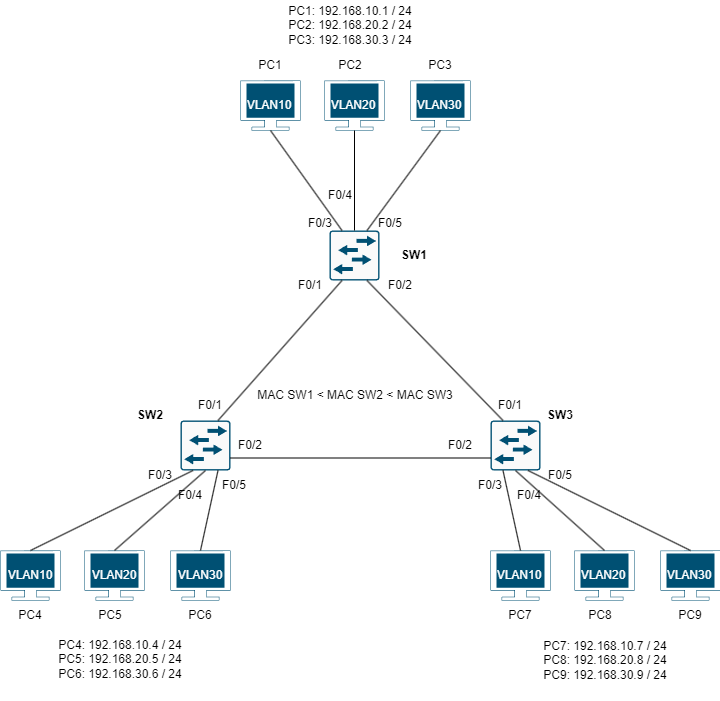
\includegraphics[width=0.8\textwidth]{img/pvst01.png}
	\caption{\textit{}}
\end{figure}


\begin{itemize}
	\item \textbf{MAC Address Order:} \\
	      \textbf{MAC SW1 $<$ MAC SW2 $<$ MAC SW3} \\
	      (SW1 has the lowest MAC address.)

	\item \textbf{VLANs and Devices:}
	      \begin{itemize}
		      \item \textbf{VLAN 10:} PC1, PC4, PC7
		      \item \textbf{VLAN 20:} PC2, PC5, PC8
		      \item \textbf{VLAN 30:} PC3, PC6, PC9
	      \end{itemize}
\end{itemize}
\newpage
\subsection*{Step-by-Step Configuration Tasks}

\begin{enumerate}

	\item \textbf{Set Inter-Switch Links to Trunk Mode} \\
	      Configure the links between the switches (\textbf{SW1, SW2, SW3}) to operate in \textbf{trunk mode} to allow VLAN traffic to pass through.

	      %---,,,,,,,,,,,,,,,,,,,,,,,,,,,,,,,,,,---
	      \switchocg{codeblock}{%
		      \color{black}\underline{Click here to display the answer:}%
	      }


	      \begin{ocg}{Code Block}{codeblock}{0}
		      \vspace{0.5cm}
		      \begin{lstlisting}
interface range f0/1 - 2
switchport mode trunk
\end{lstlisting}

	      \end{ocg}
	      %---''''''''''''''''''''''''''''''''---   
	\item \textbf{Verify Current STP Status} \\
	      Before making further changes, \textbf{check the current STP status} to see how the network has chosen the Root Bridge for each VLAN.

	      %---,,,,,,,,,,,,,,,,,,,,,,,,,,,,,,,,,,---
	      \switchocg{codeblock}{%
		      \color{black}\underline{Click here to display the answer:}%
	      }


	      \begin{ocg}{Code Block}{codeblock}{0}
		      \vspace{0.5cm}
		      \begin{lstlisting}
show spanning-tree
\end{lstlisting}

	      \end{ocg}
	      %---''''''''''''''''''''''''''''''''---  

	\item \textbf{Enable VTP on All Switches} \\
	      Configure \textbf{VTP (VLAN Trunking Protocol)} to manage VLANs centrally.

	      \textbf{VTP Settings:}
	      \begin{itemize}
		      \item \textbf{Domain Name:} \texttt{network}
		      \item \textbf{Version:} \texttt{2}
		      \item \textbf{Password:} \texttt{CCNP}
	      \end{itemize}


	      - SW1 Configuration (VTP Master/Server):

	      %---,,,,,,,,,,,,,,,,,,,,,,,,,,,,,,,,,,---
	      \switchocg{codeblock}{%
		      \color{black}\underline{Click here to display the answer:}%
	      }


	      \begin{ocg}{Code Block}{codeblock}{0}
		      \vspace{0.5cm}
		      \begin{lstlisting}
vtp domain network
vtp mode server
vtp version 2
vtp password CCNP
\end{lstlisting}

	      \end{ocg}
	      %---''''''''''''''''''''''''''''''''---

	      - SW2 and SW3 Configuration (VTP Clients):

	      %---,,,,,,,,,,,,,,,,,,,,,,,,,,,,,,,,,,---
	      \switchocg{codeblock}{%
		      \color{black}\underline{Click here to display the answer:}%
	      }


	      \begin{ocg}{Code Block}{codeblock}{0}
		      \vspace{0.5cm}
		      \begin{lstlisting}
vtp domain network
vtp mode client
vtp version 2
vtp password CCNP
\end{lstlisting}

	      \end{ocg}
	      %---''''''''''''''''''''''''''''''''---  
	\item \textbf{Create VLANs 10, 20, and 30 on SW1 (VTP Server)} \\
	      Since \textbf{SW1} is the VTP Server, create the VLANs here, and they will propagate to \textbf{SW2} and \textbf{SW3}.


	      %---,,,,,,,,,,,,,,,,,,,,,,,,,,,,,,,,,,---
	      \switchocg{codeblock}{%
		      \color{black}\underline{Click here to display the answer:}%
	      }


	      \begin{ocg}{Code Block}{codeblock}{0}
		      \vspace{0.5cm}
		      \begin{lstlisting}
vlan 10
name VLAN10
vlan 20
name VLAN20
vlan 30
name VLAN30
\end{lstlisting}

	      \end{ocg}
	      %---''''''''''''''''''''''''''''''''---


	\item \textbf{Verify STP Status After VLAN Creation} \\
	      After setting up VTP and VLANs, check how \textbf{PVST} has adjusted the spanning tree roles.


	      %---,,,,,,,,,,,,,,,,,,,,,,,,,,,,,,,,,,---
	      \switchocg{codeblock}{%
		      \color{black}\underline{Click here to display the answer:}%
	      }


	      \begin{ocg}{Code Block}{codeblock}{0}
		      \vspace{0.5cm}
		      \begin{lstlisting}
show spanning-tree vlan 10
show spanning-tree vlan 20
show spanning-tree vlan 30
\end{lstlisting}

	      \end{ocg}
	      %---''''''''''''''''''''''''''''''''---


\end{enumerate}

\section*{PVST Root Bridge Configuration Per VLAN}

\begin{enumerate}

	\item \textbf{Set Root Bridges for Each VLAN Using PVST+} \\
	      Configure different \textbf{Root Bridges} for each VLAN to optimize traffic flow:

	      \begin{itemize}
		      \item \textbf{VLAN 10 Root Bridge:} Set \textbf{SW1} as the Root Bridge.
		      \item \textbf{VLAN 20 Root Bridge:} Set \textbf{SW2} as the Root Bridge.
		      \item \textbf{VLAN 30 Root Bridge:} Set \textbf{SW3} as the Root Bridge.
	      \end{itemize}



	      - SW1 (Root for VLAN 10):

	      %---,,,,,,,,,,,,,,,,,,,,,,,,,,,,,,,,,,---
	      \switchocg{codeblock}{%
		      \color{black}\underline{Click here to display the answer:}%
	      }


	      \begin{ocg}{Code Block}{codeblock}{0}
		      \vspace{0.5cm}
		      \begin{lstlisting}
spanning-tree vlan 10 priority 4096
\end{lstlisting}

	      \end{ocg}
	      %---''''''''''''''''''''''''''''''''---
	      - SW2 (Root for VLAN 20):

	      %---,,,,,,,,,,,,,,,,,,,,,,,,,,,,,,,,,,---
	      \switchocg{codeblock}{%
		      \color{black}\underline{Click here to display the answer:}%
	      }


	      \begin{ocg}{Code Block}{codeblock}{0}
		      \vspace{0.5cm}
		      \begin{lstlisting}
spanning-tree vlan 20 priority 4096
\end{lstlisting}

	      \end{ocg}
	      %---''''''''''''''''''''''''''''''''---
	      - SW3 (Root for VLAN 30):

	      %---,,,,,,,,,,,,,,,,,,,,,,,,,,,,,,,,,,---
	      \switchocg{codeblock}{%
		      \color{black}\underline{Click here to display the answer:}%
	      }


	      \begin{ocg}{Code Block}{codeblock}{0}
		      \vspace{0.5cm}
		      \begin{lstlisting}
spanning-tree vlan 30 priority 4096
\end{lstlisting}

	      \end{ocg}
	      %---''''''''''''''''''''''''''''''''---

	      \textit{Note:} A lower priority value increases the likelihood of a switch becoming the Root Bridge. The default is 32768.

	\item \textbf{Verify STP Status After Root Bridge Configuration} \\
	      After configuring the Root Bridges for each VLAN, verify that the changes were applied correctly.

	      %---,,,,,,,,,,,,,,,,,,,,,,,,,,,,,,,,,,---
	      \switchocg{codeblock}{%
		      \color{black}\underline{Click here to display the answer:}%
	      }


	      \begin{ocg}{Code Block}{codeblock}{0}
		      \vspace{0.5cm}
		      \begin{lstlisting}
show spanning-tree vlan 10
show spanning-tree vlan 20
show spanning-tree vlan 30
\end{lstlisting}

	      \end{ocg}
	      %---''''''''''''''''''''''''''''''''---

	      \newpage
	\item \textbf{Draw the active topology of each violin.} \\
	      - SW1 (Root for VLAN 10):


	      - SW2 (Root for VLAN 20):


	      - SW3 (Root for VLAN 30):
	      \begin{figure}[h]
		      \centering
		      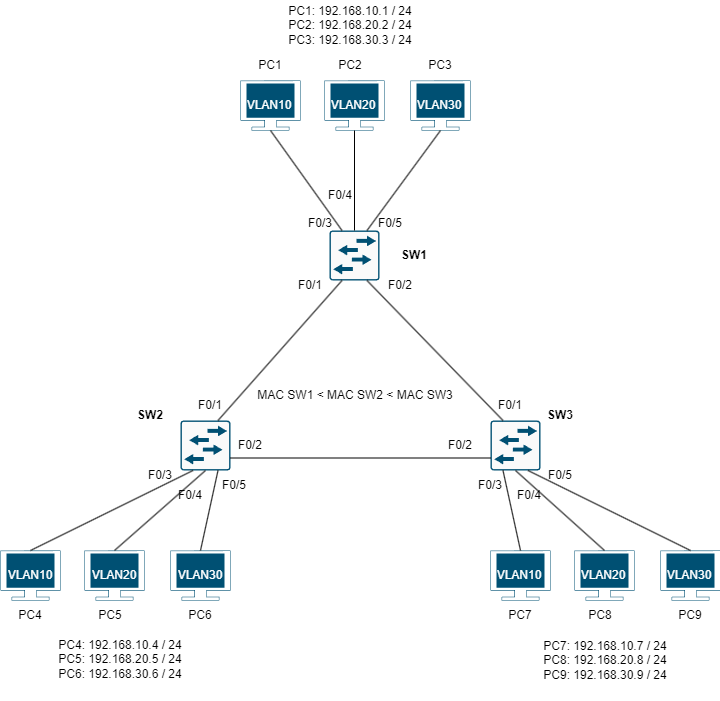
\includegraphics[width=0.8\textwidth]{img/pvst01.png}
		      \caption{\textit{}}
	      \end{figure}
\end{enumerate}
\newpage
%---,,,,,,,,,,,,,,,,,,,,,,,,,,,,,,,,,,---


\switchocg{codeblock}{
	\color{black}\underline{Click here to display the answer:}%
}

\begin{ocg}{Code Block}{codeblock}{0}

	\tcbset{colback=gray!10, colframe=gray!50, boxrule=0.5pt, arc=4pt, left=4pt, right=4pt, top=4pt, bottom=4pt, width=0.7\textwidth}
	\begin{tcolorbox}

		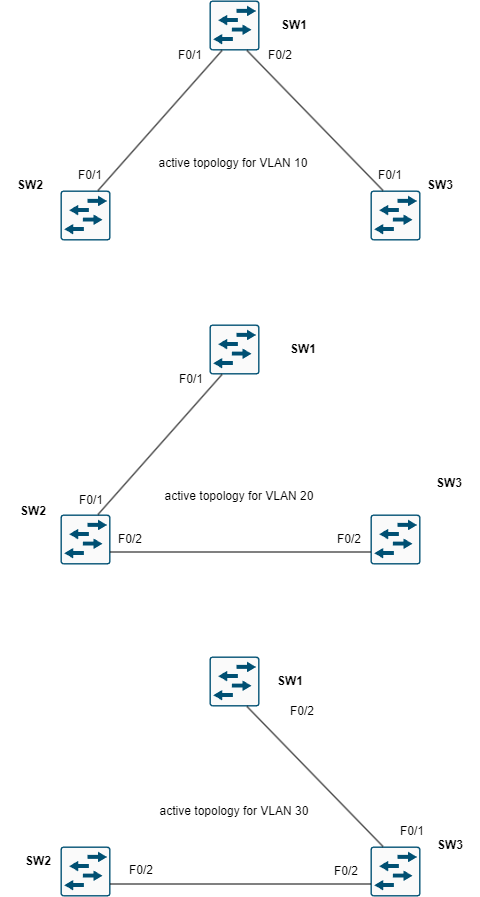
\includegraphics[width=\textwidth]{img/pvst01active.png}

	\end{tcolorbox}
\end{ocg}

%---''''''''''''''''''''''''''''''''---   
\newpage

\section*{Configure PortFast for End Devices}

\begin{enumerate}
	\item \textbf{Enable PortFast on All PC Ports} \\
	      PortFast allows end devices (like PCs) to bypass STP's listening and learning states, enabling faster connections.

	      \textit{Task:} Configure \textbf{PortFast} on interfaces connected to PCs (e.g., \textbf{F0/3}, \textbf{F0/4}, \textbf{F0/5} on SW1).


	      %---,,,,,,,,,,,,,,,,,,,,,,,,,,,,,,,,,,---
	      \switchocg{codeblock}{%
		      \color{black}\underline{Click here to display the answer:}%
	      }


	      \begin{ocg}{Code Block}{codeblock}{0}
		      \vspace{0.5cm}
		      \begin{lstlisting}
interface range f0/3 - 5
spanning-tree portfast
\end{lstlisting}

	      \end{ocg}
	      %---''''''''''''''''''''''''''''''''---

	\item \textbf{Verify Connectivity Between PC2 and PC3} \\
	      \textit{Task:} Test the connection between \textbf{PC2 (192.168.20.2)} and \textbf{PC3 (192.168.30.3)} using the \textbf{ping} command.


	\item \textbf{Enable Debugging on SW3} \\
	      Monitor STP behavior during topology changes.

	      \textit{Task:} Turn on STP debugging on \textbf{SW3}.

	      %---,,,,,,,,,,,,,,,,,,,,,,,,,,,,,,,,,,---
	      \switchocg{codeblock}{%
		      \color{black}\underline{Click here to display the answer:}%
	      }


	      \begin{ocg}{Code Block}{codeblock}{0}
		      \vspace{0.5cm}
		      \begin{lstlisting}
debug spanning-tree events
\end{lstlisting}

	      \end{ocg}
	      %---''''''''''''''''''''''''''''''''---

	\item \textbf{Shut Down Interfaces to Trigger Topology Changes} \\
	      Simulate link failures by shutting down specific interfaces:

	      \textit{Task:} Shut down \textbf{F0/1} on \textbf{SW3} and \textbf{F0/2} on \textbf{SW1}:

	      %---,,,,,,,,,,,,,,,,,,,,,,,,,,,,,,,,,,---
	      \switchocg{codeblock}{%
		      \color{black}\underline{Click here to display the answer:}%
	      }


	      \begin{ocg}{Code Block}{codeblock}{0}
		      \vspace{0.5cm}
		      \begin{itemize}
			      \item en switch SW1
			            \begin{lstlisting}
interface f0/2
shutdown
                \end{lstlisting}
			      \item en switch SW3
			            \begin{lstlisting}
interface f0/1
shutdown
                \end{lstlisting}
		      \end{itemize}
	      \end{ocg}
	      %---''''''''''''''''''''''''''''''''---
	\item \textbf{Observe and Estimate New Topology} \\
	      After shutting down the interfaces:

	      \textit{Task:} Check the \textbf{new port roles} and \textbf{STP state} using:

	      %---,,,,,,,,,,,,,,,,,,,,,,,,,,,,,,,,,,---
	      \switchocg{codeblock}{%
		      \color{black}\underline{Click here to display the answer:}%
	      }


	      \begin{ocg}{Code Block}{codeblock}{0}
		      \vspace{0.5cm}
		      \begin{lstlisting}
show spanning-tree
                \end{lstlisting}
	      \end{ocg}
	      %---''''''''''''''''''''''''''''''''---

	      \textbf{Question:} Which ports have become \textbf{Root Ports} or \textbf{Designated Ports}? Identify if any ports are now \textbf{Blocked}.

	\item \textbf{Restore the Network to Its Original State} \\
	      Re-enable the interfaces to bring the network back to its initial state.

	      \textit{Task:}  Turn on \textbf{F0/1} on \textbf{SW3} and \textbf{F0/2} on \textbf{SW1}:

	      %---,,,,,,,,,,,,,,,,,,,,,,,,,,,,,,,,,,---
	      \switchocg{codeblock}{%
		      \color{black}\underline{Click here to display the answer:}%
	      }


	      \begin{ocg}{Code Block}{codeblock}{0}
		      \vspace{0.5cm}
		      \begin{itemize}
			      \item en switch SW1
			            \begin{lstlisting}
interface f0/2
no shutdown
                \end{lstlisting}
			      \item en switch SW3
			            \begin{lstlisting}
interface f0/1
no shutdown
                \end{lstlisting}
		      \end{itemize}
	      \end{ocg}
	      %---''''''''''''''''''''''''''''''''---

	\item \textbf{Reduce Network Diameter for Faster Convergence} \\
	      The \textbf{network diameter} defines the maximum number of switches a BPDU can pass through. Reducing it speeds up convergence.

	      \textit{Task:} Reduce the \textbf{network diameter} from the default \textbf{7} to \textbf{2}.


	      %---,,,,,,,,,,,,,,,,,,,,,,,,,,,,,,,,,,---
	      \switchocg{codeblock}{%
		      \color{black}\underline{Click here to display the answer:}%
	      }


	      \begin{ocg}{Code Block}{codeblock}{0}
		      \vspace{0.5cm}
		      \begin{lstlisting}
spanning-tree vlan [VLAN-ID] diameter 2
            \end{lstlisting}
	      \end{ocg}
	      %---''''''''''''''''''''''''''''''''---
	\item \textbf{Check Forward Delay and Max Age Timers} \\
	      STP uses these timers to control how long switches stay in different states during convergence.

	      \textit{Task:} Verify \textbf{Forward Delay} and \textbf{Max Age} settings:

	      %---,,,,,,,,,,,,,,,,,,,,,,,,,,,,,,,,,,---
	      \switchocg{codeblock}{%
		      \color{black}\underline{Click here to display the answer:}%
	      }


	      \begin{ocg}{Code Block}{codeblock}{0}
		      \vspace{0.5cm}
		      \begin{lstlisting}
show spanning-tree vlan [VLAN-ID]
            \end{lstlisting}
	      \end{ocg}
	      %---''''''''''''''''''''''''''''''''---

	\item \textbf{Enable UplinkFast on SW2 for Faster Recovery} \\
	      \textbf{UplinkFast} speeds up STP convergence when a primary link fails by immediately switching to a backup link.

	      \textit{Task:} Enable \textbf{UplinkFast} on \textbf{SW2}:

	      %---,,,,,,,,,,,,,,,,,,,,,,,,,,,,,,,,,,---
	      \switchocg{codeblock}{%
		      \color{black}\underline{Click here to display the answer:}%
	      }


	      \begin{ocg}{Code Block}{codeblock}{0}
		      \vspace{0.5cm}
		      \begin{lstlisting}
spanning-tree uplinkfast
            \end{lstlisting}
	      \end{ocg}
	      %---''''''''''''''''''''''''''''''''---

	\item \textbf{Set Max-Update-Rate to 100 Packets per Second} \\
	      Limit the number of update packets sent per second to prevent excessive flooding during topology changes.

	      \textit{Task:} Set \textbf{max-update-rate} to \textbf{100 packets/sec}:

	      %---,,,,,,,,,,,,,,,,,,,,,,,,,,,,,,,,,,---
	      \switchocg{codeblock}{%
		      \color{black}\underline{Click here to display the answer:}%
	      }


	      \begin{ocg}{Code Block}{codeblock}{0}
		      \vspace{0.5cm}
		      \begin{lstlisting}
spanning-tree uplinkfast max-update-rate 100
          \end{lstlisting}
	      \end{ocg}
	      %---''''''''''''''''''''''''''''''''---
	\item \textbf{Verify Uplink Status on SW2} \\
	      \textit{Task:} Check if \textbf{UplinkFast} is working correctly:

	      %---,,,,,,,,,,,,,,,,,,,,,,,,,,,,,,,,,,---
	      \switchocg{codeblock}{%
		      \color{black}\underline{Click here to display the answer:}%
	      }


	      \begin{ocg}{Code Block}{codeblock}{0}
		      \vspace{0.5cm}
		      \begin{lstlisting}
show spanning-tree uplinkfast
          \end{lstlisting}
	      \end{ocg}
	      %---''''''''''''''''''''''''''''''''---

\end{enumerate}

\chapter{Protecting the Spanning Tree Protocol (STP) Topology}


\noindent The \textbf{Spanning Tree Protocol (STP)} is crucial for maintaining a loop-free and stable Layer 2 network topology. However, without proper safeguards, STP can become vulnerable to misconfigurations or malicious attacks, potentially leading to network loops, instability, or even downtime. To enhance the security and stability of the STP topology, network administrators can implement various protection mechanisms, including \textbf{BPDU Guard}, \textbf{Root Guard}, \textbf{BPDU Filter}, \textbf{Loop Guard}, and \textbf{UDLD (Unidirectional Link Detection)}. These features help prevent unauthorized devices from influencing STP operations, detect unidirectional links, and ensure consistent network behavior.

\section*{BPDU Guard}

\textbf{Bridge Protocol Data Units (BPDUs)} are essential messages exchanged between switches to maintain the STP topology. \textbf{BPDU Guard} is a protective feature designed to secure \textbf{PortFast}-enabled ports, which are typically connected to end devices like computers or printers. Since these ports bypass STP’s usual listening and learning states to achieve faster connectivity, receiving BPDUs on them could indicate a misconfiguration or an attack (such as connecting a rogue switch).

When \textbf{BPDU Guard} is enabled and a BPDU is received on a PortFast port, the switch immediately \textbf{disables} the port by placing it into an \textbf{err-disabled} (error-disabled) state. This action prevents potential network loops and unauthorized participation in the STP topology. BPDU Guard is particularly useful in access layer switches where end devices should never send BPDUs.

\section*{Root Guard}

The \textbf{Root Bridge} plays a central role in STP, determining the best loop-free paths for traffic. If an unauthorized switch with a \textbf{lower Bridge ID} (priority + MAC address) is connected to the network, it could inadvertently or maliciously become the Root Bridge, altering the topology and potentially degrading network performance.

\textbf{Root Guard} prevents this by restricting specific ports from becoming Root Ports. When enabled on a port, if a superior BPDU (indicating a better Root Bridge) is received, the port is placed into a \textbf{root-inconsistent} state, effectively blocking it from influencing the Root Bridge election. Once the superior BPDUs stop, the port automatically returns to normal operation. Root Guard is typically applied on ports where no upstream Root Bridge should be allowed, such as those connecting to access layer switches.

\section*{BPDU Filter}

While \textbf{BPDU Guard} reacts to unexpected BPDUs, \textbf{BPDU Filter} prevents BPDUs from being sent or received on specific ports altogether. This feature can be applied globally or on a per-port basis:

\begin{itemize}
	\item \textbf{Globally:} BPDU Filter allows initial BPDUs to be sent when a port comes up but suppresses further BPDU exchange, making the port behave as if STP is disabled.
	\item \textbf{Per-Port:} When applied directly to a port, BPDU Filter prevents all BPDUs from being sent or received, effectively removing the port from STP participation.
\end{itemize}

\textbf{Caution:} Improper use of BPDU Filter can lead to \textbf{network loops}, as the port is unaware of STP topology changes. It should be used in controlled environments where the risk of loops is minimal.

\section*{Loop Guard}

\textbf{Loop Guard} is designed to prevent loops caused by \textbf{unidirectional link failures} in STP. In normal operation, a port in a \textbf{blocking} or \textbf{root port} state relies on receiving BPDUs from neighboring switches to maintain its status. If BPDUs unexpectedly stop arriving due to a failure, the port might incorrectly transition to the \textbf{forwarding} state, creating a loop.

When \textbf{Loop Guard} is enabled, if a port stops receiving BPDUs on a \textbf{non-designated port} (i.e., a blocking or root port), the port enters a \textbf{loop-inconsistent} state instead of transitioning to forwarding. This proactive measure prevents loops by ensuring ports stay in a safe state until the issue is resolved. Loop Guard is particularly useful on redundant links where unidirectional failures could silently cause loops.

\section*{UDLD (Unidirectional Link Detection)}

\textbf{Unidirectional Link Detection (UDLD)} is a Layer 2 protocol that detects unidirectional physical link failures, which can lead to network loops or black holes. Such failures occur when traffic flows in one direction but not the other, often due to fiber optic issues, hardware faults, or misconfigurations.

UDLD operates by exchanging \textbf{hello packets} between devices on both ends of a link. If one device stops receiving these packets while still sending its own, UDLD detects the inconsistency. Depending on the mode:
\begin{itemize}
	\item In \textbf{normal mode}, UDLD alerts administrators but does not take immediate action.
	\item In \textbf{aggressive mode}, UDLD automatically \textbf{disables} the affected port to prevent potential loops.
\end{itemize}

UDLD is particularly important in fiber optic networks, where physical link issues might not be immediately evident.

\section*{Conclusion}

Securing the \textbf{Spanning Tree Protocol} topology is essential for maintaining a reliable and stable network. Features like \textbf{BPDU Guard} and \textbf{Root Guard} prevent unauthorized devices from influencing the STP topology, while \textbf{BPDU Filter} and \textbf{Loop Guard} ensure proper BPDU handling and loop prevention. Additionally, \textbf{UDLD} plays a critical role in detecting and mitigating unidirectional link failures. By implementing these protective mechanisms, network administrators can significantly enhance the robustness and resilience of their Layer 2 networks, reducing the risk of outages, loops, and other network disruptions.


\newpage
\section*{Lab Exercises: Protecting the Spanning Tree Protocol Topology}

\begin{figure}[h]
	\centering
	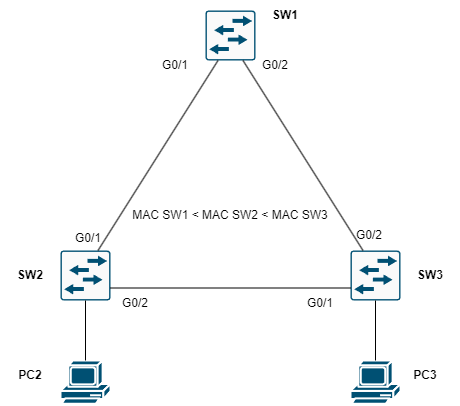
\includegraphics[width=0.8\textwidth]{img/STPConvergence01.png}
	\caption{\textit{}}
\end{figure}

\subsection*{Network Topology Overview:}

\begin{itemize}
	\item \textbf{SW1} is connected to \textbf{SW2} and \textbf{SW3}.
	\item \textbf{SW2} is connected to \textbf{PC2} and has a direct link to \textbf{SW3}.
	\item \textbf{SW3} is connected to \textbf{PC3}.
	\item \textbf{MAC Address Order:} \\
	      \textbf{MAC SW1 $<$ MAC SW2 $<$ MAC SW3} \\
	      (SW1 has the lowest MAC address and will likely become the Root Bridge unless configured otherwise.)
\end{itemize}

\subsection*{Configuring BPDU Guard}

\textbf{Objective:} Protect access ports from unauthorized devices sending BPDUs, which could cause topology changes.

\begin{enumerate}
	\item \textbf{Enable BPDU Guard on Access Ports (Connected to PCs):} \\
	      Since \textbf{PC2} and \textbf{PC3} are end devices, their interfaces should not receive BPDUs. If a BPDU is received, BPDU Guard will shut down the port to prevent loops.

	      On SW2 (Port connected to PC2) and SW3 (Port connected to PC3):


	      %---,,,,,,,,,,,,,,,,,,,,,,,,,,,,,,,,,,---
	      \switchocg{codeblock}{%
		      \color{black}\underline{Click here to display the answer:}%
	      }


	      \begin{ocg}{Code Block}{codeblock}{0}
		      \vspace{0.5cm}
		      \begin{itemize}
			      \item en switch SW2
			            \begin{lstlisting}
interface f0/1
spanning-tree portfast
spanning-tree bpduguard enable
                \end{lstlisting}
			      \item en switch SW3
			            \begin{lstlisting}
interface f0/1
spanning-tree portfast
spanning-tree bpduguard enable
                \end{lstlisting}
		      \end{itemize}
	      \end{ocg}
	      %---''''''''''''''''''''''''''''''''---


	\item \textbf{Test the Configuration:} \\
	      Connect a switch (instead of a PC) to \textbf{G0/2} on \textbf{SW2} and send BPDUs.

	      \textbf{Expected Result:} The port should move to an \textbf{err-disabled} state. Verify using:
	      %---,,,,,,,,,,,,,,,,,,,,,,,,,,,,,,,,,,---
	      \switchocg{codeblock}{%
		      \color{black}\underline{Click here to display the answer:}%
	      }


	      \begin{ocg}{Code Block}{codeblock}{0}
		      \vspace{0.5cm}
		      \begin{lstlisting}
show interface status
                \end{lstlisting}
	      \end{ocg}
	      %---''''''''''''''''''''''''''''''''---

	\item \textbf{Recover the Port:}

	      %---,,,,,,,,,,,,,,,,,,,,,,,,,,,,,,,,,,---
	      \switchocg{codeblock}{%
		      \color{black}\underline{Click here to display the answer:}%
	      }


	      \begin{ocg}{Code Block}{codeblock}{0}
		      \vspace{0.5cm}
		      \begin{itemize}
			      \item en switch SW2
			            \begin{lstlisting}
interface f0/1
shutdown
no shutdown
                \end{lstlisting}
			      \item en switch SW3
			            \begin{lstlisting}
interface f0/1
shutdown
no shutdown
                \end{lstlisting}
		      \end{itemize}
	      \end{ocg}
	      %---''''''''''''''''''''''''''''''''---
\end{enumerate}

\subsection*{Configuring Root Guard}

\textbf{Objective:} Prevent unauthorized switches from becoming the Root Bridge.

\begin{enumerate}
	\item \textbf{Enable Root Guard on Specific Ports:} \\
	      To ensure \textbf{SW1} remains the Root Bridge, apply Root Guard on \textbf{SW2} and \textbf{SW3} ports facing other switches.

	      On SW2 (Facing SW3) and SW3 (Facing SW2):

	      %---,,,,,,,,,,,,,,,,,,,,,,,,,,,,,,,,,,---
	      \switchocg{codeblock}{%
		      \color{black}\underline{Click here to display the answer:}%
	      }


	      \begin{ocg}{Code Block}{codeblock}{0}
		      \vspace{0.5cm}
		      \begin{itemize}
			      \item en switch SW2
			            \begin{lstlisting}
interface f0/1
spanning-tree guard root
                \end{lstlisting}
			      \item en switch SW3
			            \begin{lstlisting}
interface f0/1
spanning-tree guard root
                \end{lstlisting}
		      \end{itemize}
	      \end{ocg}
	      %---''''''''''''''''''''''''''''''''---

	\item \textbf{Test the Configuration:} \\
	      Lower the bridge priority on \textbf{SW3} to try to make it the Root Bridge:

	      %---,,,,,,,,,,,,,,,,,,,,,,,,,,,,,,,,,,---
	      \switchocg{codeblock}{%
		      \color{black}\underline{Click here to display the answer:}%
	      }


	      \begin{ocg}{Code Block}{codeblock}{0}
		      \vspace{0.5cm}
		      \begin{lstlisting}
spanning-tree vlan 1 priority 4096
                \end{lstlisting}
	      \end{ocg}
	      %---''''''''''''''''''''''''''''''''---
	      \textit{Expected Result:} The port on \textbf{SW2} connected to \textbf{SW3} should go into a \textbf{root-inconsistent} state, preventing \textbf{SW3} from becoming the Root Bridge.

	\item \textbf{Verify the Root Guard Status:}

	      %---,,,,,,,,,,,,,,,,,,,,,,,,,,,,,,,,,,---
	      \switchocg{codeblock}{%
		      \color{black}\underline{Click here to display the answer:}%
	      }


	      \begin{ocg}{Code Block}{codeblock}{0}
		      \vspace{0.5cm}
		      \begin{lstlisting}
show spanning-tree inconsistentports
                \end{lstlisting}
	      \end{ocg}
	      %---''''''''''''''''''''''''''''''''---
\end{enumerate}





\section*{Exercise 3: Configuring BPDU Filter}

\textbf{Objective:} Suppress BPDU transmission on specific ports to prevent unnecessary STP participation.

\begin{enumerate}
	\item \textbf{Enable BPDU Filter on Access Ports (Connected to PCs):}

	      \textbf{On SW2 (Port connected to PC2):}

	      %---,,,,,,,,,,,,,,,,,,,,,,,,,,,,,,,,,,---
	      \switchocg{codeblock}{%
		      \color{black}\underline{Click here to display the answer:}%
	      }


	      \begin{ocg}{Code Block}{codeblock}{0}
		      \vspace{0.5cm}
		      \begin{lstlisting}
interface f0/2
spanning-tree bpdufilter enable
            \end{lstlisting}
	      \end{ocg}
	      %---''''''''''''''''''''''''''''''''---


	      \textbf{On SW3 (Port connected to PC3):}

	      %---,,,,,,,,,,,,,,,,,,,,,,,,,,,,,,,,,,---
	      \switchocg{codeblock}{%
		      \color{black}\underline{Click here to display the answer:}%
	      }


	      \begin{ocg}{Code Block}{codeblock}{0}
		      \vspace{0.5cm}
		      \begin{lstlisting}
interface f0/1
spanning-tree bpdufilter enable
\end{lstlisting}
	      \end{ocg}
	      %---''''''''''''''''''''''''''''''''---

	\item \textbf{Test the Configuration:} \\
	      Verify that BPDUs are not being sent on these interfaces:

	      %---,,,,,,,,,,,,,,,,,,,,,,,,,,,,,,,,,,---
	      \switchocg{codeblock}{%
		      \color{black}\underline{Click here to display the answer:}%
	      }


	      \begin{ocg}{Code Block}{codeblock}{0}
		      \vspace{0.5cm}
		      \begin{lstlisting}
debug spanning-tree bpdu send
    \end{lstlisting}
	      \end{ocg}
	      %---''''''''''''''''''''''''''''''''---

	\item \textbf{Warning:} \\
	      \textbf{BPDU Filter} disables STP on the interface, which can lead to network loops if a switch is accidentally connected.
\end{enumerate}

\section*{Exercise 4: Configuring Loop Guard}

\textbf{Objective:} Prevent loops caused by unidirectional link failures in the STP topology.

\begin{enumerate}
	\item \textbf{Enable Loop Guard on Non-Designated Ports:} \\
	      Loop Guard should be applied to \textbf{root ports} and \textbf{alternate ports} that might stop receiving BPDUs.

	      \textbf{On SW2 and SW3 (Ports facing SW1):}

	      %---,,,,,,,,,,,,,,,,,,,,,,,,,,,,,,,,,,---
	      \switchocg{codeblock}{%
		      \color{black}\underline{Click here to display the answer:}%
	      }


	      \begin{ocg}{Code Block}{codeblock}{0}
		      \vspace{0.5cm}
		      \begin{itemize}
			      \item en switch SW2
			            \begin{lstlisting}
interface g0/1
spanning-tree guard loop
                \end{lstlisting}
			      \item en switch SW3
			            \begin{lstlisting}
interface g0/2
spanning-tree guard loop
                \end{lstlisting}
		      \end{itemize}
	      \end{ocg}
	      %---''''''''''''''''''''''''''''''''---

	\item \textbf{Simulate a Unidirectional Link Failure:} \\
	      Disconnect the \textbf{TX (Transmit)} fiber cable from \textbf{SW1’s G0/1} while keeping \textbf{RX (Receive)} connected.

	      \textbf{Expected Result:} The port on \textbf{SW2} should enter a \textbf{loop-inconsistent} state instead of transitioning to forwarding.

	\item \textbf{Verify Loop Guard Status:}

	      %---,,,,,,,,,,,,,,,,,,,,,,,,,,,,,,,,,,---
	      \switchocg{codeblock}{%
		      \color{black}\underline{Click here to display the answer:}%
	      }


	      \begin{ocg}{Code Block}{codeblock}{0}
		      \vspace{0.5cm}
		      \begin{lstlisting}
show spanning-tree inconsistentports
    \end{lstlisting}
	      \end{ocg}
	      %---''''''''''''''''''''''''''''''''---
\end{enumerate}

\section*{Exercise 5: Configuring UDLD (Unidirectional Link Detection)}

\textbf{Objective:} Detect and disable unidirectional links to prevent loops.

\begin{enumerate}
	\item \textbf{Enable UDLD on Fiber Links Between Switches:} \\
	      Apply UDLD on the \textbf{G0/1} and \textbf{G0/2} interfaces between switches.

	      \textbf{On SW1:}

	      %---,,,,,,,,,,,,,,,,,,,,,,,,,,,,,,,,,,---
	      \switchocg{codeblock}{%
		      \color{black}\underline{Click here to display the answer:}%
	      }


	      \begin{ocg}{Code Block}{codeblock}{0}
		      \vspace{0.5cm}
		      \begin{lstlisting}
interface range g0/1 - 2
udld aggressive
    \end{lstlisting}
	      \end{ocg}
	      %---''''''''''''''''''''''''''''''''---

	      \textbf{On SW2 and SW3 (Interfaces facing SW1):}

	      %---,,,,,,,,,,,,,,,,,,,,,,,,,,,,,,,,,,---
	      \switchocg{codeblock}{%
		      \color{black}\underline{Click here to display the answer:}%
	      }


	      \begin{ocg}{Code Block}{codeblock}{0}
		      \vspace{0.5cm}
		      \begin{itemize}
			      \item en switch SW2
			            \begin{lstlisting}
interface g0/1
udld aggressive
                \end{lstlisting}
			      \item en switch SW3
			            \begin{lstlisting}
interface g0/2
udld aggressive
                \end{lstlisting}
		      \end{itemize}
	      \end{ocg}
	      %---''''''''''''''''''''''''''''''''---

	\item \textbf{Test UDLD Functionality:} \\
	      Disconnect one side of the fiber link (e.g., \textbf{TX} on \textbf{SW1 G0/1}).

	      \textbf{Expected Result:} UDLD will detect the unidirectional link and place the port in an \textbf{err-disabled} state.

	\item \textbf{Verify UDLD Status:}

	      %---,,,,,,,,,,,,,,,,,,,,,,,,,,,,,,,,,,---
	      \switchocg{codeblock}{%
		      \color{black}\underline{Click here to display the answer:}%
	      }


	      \begin{ocg}{Code Block}{codeblock}{0}
		      \vspace{0.5cm}
		      \begin{lstlisting}
show udld interface
    \end{lstlisting}
	      \end{ocg}
	      %---''''''''''''''''''''''''''''''''---

	\item \textbf{Recover UDLD-disabled Ports:}

	      %---,,,,,,,,,,,,,,,,,,,,,,,,,,,,,,,,,,---
	      \switchocg{codeblock}{%
		      \color{black}\underline{Click here to display the answer:}%
	      }


	      \begin{ocg}{Code Block}{codeblock}{0}
		      \vspace{0.5cm}
		      \begin{itemize}
			      \item en switch SW2
			            \begin{lstlisting}
interface g0/1  
udld reset
                \end{lstlisting}
			      \item en switch SW3
			            \begin{lstlisting}
interface g0/2
udld reset
                \end{lstlisting}
		      \end{itemize}
	      \end{ocg}
	      %---''''''''''''''''''''''''''''''''---
\end{enumerate}

\section*{Discussion Questions:}

\begin{enumerate}
	\item What happens when BPDU Guard is triggered? How is this different from BPDU Filter?
	\item How does Root Guard prevent unauthorized topology changes, and in what scenarios would it be most useful?
	\item What is the difference between Loop Guard and UDLD in handling unidirectional link failures?
	\item After enabling UDLD, how quickly did the network detect and respond to a unidirectional failure compared to standard STP behavior?
\end{enumerate}


\chapter{Rapid Per-VLAN Spanning Tree (Rapid PVST)}




\section*{Introduction to Rapid PVST}
Rapid Per-VLAN Spanning Tree (\textbf{Rapid PVST}) is a Cisco proprietary enhancement of the Spanning Tree Protocol (STP) that operates per VLAN while incorporating the rapid convergence benefits of Rapid Spanning Tree Protocol (RSTP). Rapid PVST allows each VLAN to have its own independent spanning tree instance, providing greater flexibility and network optimization in Layer 2 networks.

\section*{Key Features of Rapid PVST}
\begin{itemize}
	\item \textbf{Per-VLAN Instance:} Unlike standard RSTP, which runs a single instance for the entire network, Rapid PVST maintains a separate spanning tree for each VLAN, allowing better load balancing and path optimization.
	\item \textbf{Rapid Convergence:} By leveraging RSTP (802.1w) mechanisms, Rapid PVST provides faster recovery from topology changes compared to traditional STP (802.1D).
	\item \textbf{Port Roles \& States:} Rapid PVST uses the same port roles as RSTP—Root, Designated, Alternate, and Backup—ensuring efficient network operation with minimal downtime.
	\item \textbf{BPDU Exchange:} Bridge Protocol Data Units (BPDUs) are sent out every hello interval (default: 2 seconds) on all ports, enabling rapid detection of topology changes.
	\item \textbf{Backwards Compatibility:} Rapid PVST can interoperate with traditional STP but may fall back to legacy STP behavior if necessary.
\end{itemize}

\section*{Advantages of Rapid PVST}
\begin{enumerate}
	\item \textbf{Faster Convergence} – Utilizes rapid transition mechanisms like Proposal/Agreement handshaking for faster network recovery.
	\item \textbf{Enhanced Load Balancing} – By running a separate instance for each VLAN, traffic can be distributed efficiently across different spanning trees.
	\item \textbf{Loop Prevention} – Maintains a loop-free topology by dynamically adjusting port states in response to network topology changes.
	\item \textbf{Optimized Network Performance} – By isolating VLANs, network resources are used efficiently, reducing unnecessary traffic forwarding.
\end{enumerate}

\section*{Configuring Rapid PVST on Cisco Switches}
To enable Rapid PVST on a Cisco switch, use the following command in global configuration mode:

\begin{lstlisting}
Switch(config)# spanning-tree mode rapid-pvst
\end{lstlisting}

To configure a switch as the root bridge for a specific VLAN:

\begin{lstlisting}
Switch(config)# spanning-tree vlan <VLAN_ID> root primary
\end{lstlisting}

To adjust the bridge priority for better root bridge election control:

\begin{lstlisting}
Switch(config)# spanning-tree vlan <VLAN_ID> priority <value>
\end{lstlisting}

(Default priority is 32768, lower values increase priority.)

\section*{Conclusion}
Rapid PVST enhances the traditional Spanning Tree Protocol by providing per-VLAN instances with rapid convergence benefits. It is an essential protocol for networks requiring fast recovery, load balancing, and improved performance across multiple VLANs. Understanding and implementing Rapid PVST effectively ensures a stable and efficient Layer 2 topology in enterprise networks.



\newpage


\section*{Lab Exercises: Rapid Per-VLAN Spanning Tree}


\subsection{Network Topology Overview}

The network topology consists of four switches (SW1, SW2, SW3, and SW4) and four personal computers (PC1, PC2, PC3, and PC4). The switches are interconnected in a redundant manner, forming a robust network infrastructure to ensure reliability and fault tolerance.
\begin{figure}[h]
	\centering
	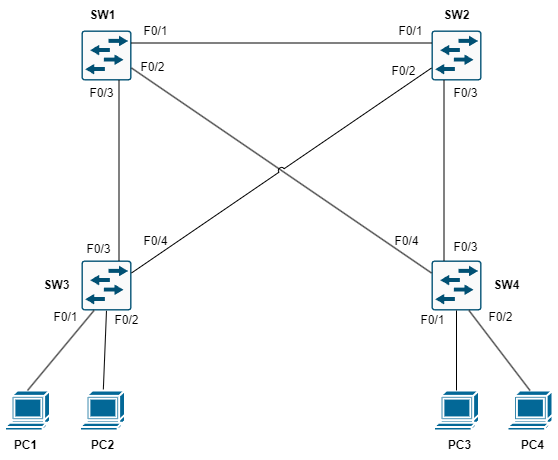
\includegraphics[width=0.8\textwidth]{img/rstp.png}
	\caption{\textit{}}
\end{figure}

\begin{enumerate}
	\item \textbf{Enable RSTP on All Switches}
	      \begin{itemize}
		      \item Configure \textbf{RSTP (Rapid PVST+)} on all switches in this topology.
		      \item Verify that RSTP is running correctly.
	      \end{itemize}
	      %---,,,,,,,,,,,,,,,,,,,,,,,,,,,,,,,,,,---
	      \switchocg{codeblock}{%
		      \color{black}\underline{Click here to display the answer:}%
	      }


	      \begin{ocg}{Code Block}{codeblock}{0}
		      \vspace{0.5cm}
		      \begin{lstlisting}
conf t
spanning-tree mode rapid-pvst
end
show spanning-tree
                    \end{lstlisting}
	      \end{ocg}
	      %---''''''''''''''''''''''''''''''''---


	      \textbf{Question:} What is the current \textbf{Root Bridge}, and how was it selected?


	      %---,,,,,,,,,,,,,,,,,,,,,,,,,,,,,,,,,,---
	      \switchocg{codeblock}{%
		      \color{black}\underline{Click here to display the answer:}%
	      }


	      \begin{ocg}{Code Block}{codeblock}{0}
		      \vspace{0.5cm}
		      \begin{itemize}
			      \item The \textbf{Root Bridge} is selected based on the \textbf{lowest Bridge ID} (combination of priority and MAC address).
			      \item By default, the switch with the \textbf{lowest MAC address} becomes the Root Bridge if all switches have the same priority (default: \textbf{32768}).
			      \item We can verify this with:
		      \end{itemize}
		      \begin{lstlisting}
show spanning-tree vlan 1
              \end{lstlisting}
	      \end{ocg}
	      %---''''''''''''''''''''''''''''''''---

	\item \textbf{Manually Set SW1 as the Root Bridge}
	      \begin{itemize}
		      \item Configure \textbf{SW1} as the \textbf{Root Bridge} for VLAN 1.
		      \item Verify that SW1 is now the Root Bridge.
	      \end{itemize}

	      %---,,,,,,,,,,,,,,,,,,,,,,,,,,,,,,,,,,---
	      \switchocg{codeblock}{%
		      \color{black}\underline{Click here to display the answer:}%
	      }


	      \begin{ocg}{Code Block}{codeblock}{0}
		      \vspace{0.5cm}
		      \begin{lstlisting}
conf t
spanning-tree vlan 1 priority 4096
end
show spanning-tree vlan 1
          \end{lstlisting}
	      \end{ocg}
	      %---''''''''''''''''''''''''''''''''---


	\item \textbf{Configure Edge Ports for Faster PC Connectivity}
	      \begin{itemize}
		      \item Enable \textbf{PortFast} on all PC-connected ports (\textbf{SW3 \& SW4}).
		      \item Test if these ports enter \textbf{forwarding state} immediately after connecting a device.
	      \end{itemize}

	      %---,,,,,,,,,,,,,,,,,,,,,,,,,,,,,,,,,,---
	      \switchocg{codeblock}{%
		      \color{black}\underline{Click here to display the answer:}%
	      }


	      \begin{ocg}{Code Block}{codeblock}{0}
		      \vspace{0.5cm}
		      \begin{lstlisting}
interface range f0/1 - 2
spanning-tree portfast
end
show spanning-tree interface f0/1 detail
 \end{lstlisting}
	      \end{ocg}
	      %---''''''''''''''''''''''''''''''''---

	      \textbf{Question:} Why is PortFast useful, and why shouldn’t it be used on switch-to-switch links?

	      %---,,,,,,,,,,,,,,,,,,,,,,,,,,,,,,,,,,---
	      \switchocg{codeblock}{%
		      \color{black}\underline{Click here to display the answer:}%
	      }


	      \begin{ocg}{Code Block}{codeblock}{0}
		      \vspace{0.5cm}
		      \begin{itemize}
			      \item \textbf{PortFast allows ports connected to PCs to skip the Listening/Learning STP states and immediately enter Forwarding.}
			      \item This is useful because PCs do not participate in STP, so waiting for STP transitions is unnecessary.
			      \item \textbf{PortFast should not be used on switch-to-switch links} because it disables STP protection, potentially causing loops.
		      \end{itemize}
	      \end{ocg}
	      %---''''''''''''''''''''''''''''''''---

	\item \textbf{Simulate a Link Failure and Observe RSTP Recovery}
	      \begin{itemize}
		      \item \textbf{Shutdown the link} between \textbf{SW1 and SW2}, then observe how RSTP reacts.
		      \item Which ports change their role to compensate for the failure?
	      \end{itemize}
	      %---,,,,,,,,,,,,,,,,,,,,,,,,,,,,,,,,,,---
	      \switchocg{codeblock}{%
		      \color{black}\underline{Click here to display the answer:}%
	      }


	      \begin{ocg}{Code Block}{codeblock}{0}
		      \vspace{0.5cm}
		      \begin{lstlisting}
interface f0/1
shutdown
end
show spanning-tree
 \end{lstlisting}
	      \end{ocg}
	      %---''''''''''''''''''''''''''''''''---

	      \textbf{Question:} How fast did RSTP reconverge compared to classic STP (50s convergence)?

	      %---,,,,,,,,,,,,,,,,,,,,,,,,,,,,,,,,,,---
	      \switchocg{codeblock}{%
		      \color{black}\underline{Click here to display the answer:}%
	      }


	      \begin{ocg}{Code Block}{codeblock}{0}
		      \vspace{0.5cm}
		      \begin{itemize}
			      \item Classic \textbf{STP takes 50 seconds} to reconverge (Listening: 15s, Learning: 15s, Max Age: 20s).
			      \item \textbf{RSTP converges in 1-2 seconds} using the \textbf{Proposal-Agreement mechanism}.
		      \end{itemize}
	      \end{ocg}
	      %---''''''''''''''''''''''''''''''''---



	\item \textbf{Observe the Proposal-Agreement Process in RSTP}
	      \begin{itemize}
		      \item Enable \textbf{debugging} to watch the RSTP \textbf{Proposal-Agreement} process.
	      \end{itemize}

	      %---,,,,,,,,,,,,,,,,,,,,,,,,,,,,,,,,,,---
	      \switchocg{codeblock}{%
		      \color{black}\underline{Click here to display the answer:}%
	      }


	      \begin{ocg}{Code Block}{codeblock}{0}
		      \vspace{0.5cm}
		      \begin{lstlisting}
debug spanning-tree events
              \end{lstlisting}
	      \end{ocg}
	      %---''''''''''''''''''''''''''''''''---

	      \textbf{Question:} What happens when a switch detects a new Root Bridge or topology change?


	      %---,,,,,,,,,,,,,,,,,,,,,,,,,,,,,,,,,,---
	      \switchocg{codeblock}{%
		      \color{black}\underline{Click here to display the answer:}%
	      }


	      \begin{ocg}{Code Block}{codeblock}{0}
		      \vspace{0.5cm}
		      \begin{itemize}
			      \item \textbf{RSTP Proposal-Agreement Process:}
			            \begin{enumerate}
				            \item A switch detects a better Root Bridge or a topology change.
				            \item It \textbf{sends a Proposal BPDU} to its neighbor.
				            \item The neighbor \textbf{temporarily blocks non-root ports}, processes the change, then sends an \textbf{Agreement BPDU} back.
				            \item The original switch transitions the link to Forwarding.
			            \end{enumerate}
			      \item This is much faster than classic STP.
		      \end{itemize}
	      \end{ocg}
	      %---''''''''''''''''''''''''''''''''---


	      \textbf{Disable Debugging (After Observation):}

	      %---,,,,,,,,,,,,,,,,,,,,,,,,,,,,,,,,,,---
	      \switchocg{codeblock}{%
		      \color{black}\underline{Click here to display the answer:}%
	      }


	      \begin{ocg}{Code Block}{codeblock}{0}
		      \vspace{0.5cm}
		      \begin{lstlisting}
undebug all
              \end{lstlisting}
	      \end{ocg}
	      %---''''''''''''''''''''''''''''''''---


	\item \textbf{Reduce the Network Diameter to Speed Up Convergence}
	      \begin{itemize}
		      \item Lower the STP \textbf{diameter} value to \textbf{2} to speed up BPDU propagation.
	      \end{itemize}

	      %---,,,,,,,,,,,,,,,,,,,,,,,,,,,,,,,,,,---
	      \switchocg{codeblock}{%
		      \color{black}\underline{Click here to display the answer:}%
	      }


	      \begin{ocg}{Code Block}{codeblock}{0}
		      \vspace{0.5cm}
		      \begin{lstlisting}
spanning-tree vlan 1 root primary diameter 2
end
show spanning-tree detail
              \end{lstlisting}
	      \end{ocg}
	      %---''''''''''''''''''''''''''''''''---

	      \textbf{Question:} How does reducing the network diameter affect STP timers?
	      %---,,,,,,,,,,,,,,,,,,,,,,,,,,,,,,,,,,---
	      \switchocg{codeblock}{%
		      \color{black}\underline{Click here to display the answer:}%
	      }


	      \begin{ocg}{Code Block}{codeblock}{0}
		      \vspace{0.5cm}
		      \begin{itemize}
			      \item The \textbf{default STP diameter is 7}, which affects BPDU propagation delays.
			      \item Reducing the \textbf{diameter to 2 speeds up convergence} because fewer hops exist.
		      \end{itemize}

		      \textbf{Verification Command:}
		      \begin{lstlisting}
show spanning-tree detail
                \end{lstlisting}
	      \end{ocg}
	      %---''''''''''''''''''''''''''''''''---




	\item \textbf{Adjust STP Timers for Faster Convergence}
	      \begin{itemize}
		      \item Reduce the \textbf{Forward Delay} and \textbf{Max Age} timers to optimize RSTP performance.
	      \end{itemize}

	      %---,,,,,,,,,,,,,,,,,,,,,,,,,,,,,,,,,,---
	      \switchocg{codeblock}{%
		      \color{black}\underline{Click here to display the answer:}%
	      }


	      \begin{ocg}{Code Block}{codeblock}{0}
		      \vspace{0.5cm}
		      \begin{lstlisting}
spanning-tree vlan 1 forward-time 10
spanning-tree vlan 1 max-age 15
end
show spanning-tree detail
              \end{lstlisting}
	      \end{ocg}
	      %---''''''''''''''''''''''''''''''''---



	\item \textbf{Configure UplinkFast on SW3 and SW4}
	      \begin{itemize}
		      \item Allow \textbf{faster failover} when a Root Port fails.
	      \end{itemize}

	      %---,,,,,,,,,,,,,,,,,,,,,,,,,,,,,,,,,,---
	      \switchocg{codeblock}{%
		      \color{black}\underline{Click here to display the answer:}%
	      }


	      \begin{ocg}{Code Block}{codeblock}{0}
		      \vspace{0.5cm}
		      \begin{lstlisting}
spanning-tree uplinkfast
end
show spanning-tree uplinkfast
    \end{lstlisting}
	      \end{ocg}
	      %---''''''''''''''''''''''''''''''''---


	      \textbf{Test:} Disable the primary Root Port and see how quickly the \textbf{backup link} takes over.

\end{enumerate}


\chapter{Multiple Spanning Tree (MST)}


\section*{Introduction to MST}
Multiple Spanning Tree (\textbf{MST}) is an advanced version of the Spanning Tree Protocol (\textbf{STP}) that allows multiple VLANs to be mapped to a single spanning tree instance. MST is standardized under \textbf{IEEE 802.1s} and provides a scalable, efficient way to manage Layer 2 network redundancy while optimizing network performance.

\section*{Key Features of MST}
\begin{itemize}
	\item \textbf{Instance-Based Spanning Trees:} Unlike Per-VLAN Spanning Tree (\textbf{PVST+} and \textbf{Rapid PVST}), which creates a separate spanning tree instance for each VLAN, MST groups multiple VLANs into a single spanning tree instance (\textbf{MSTI}), reducing CPU and memory overhead on network devices.
	\item \textbf{Improved Scalability:} Since fewer spanning tree instances run in the network, MST significantly reduces processing overhead compared to PVST+ or Rapid PVST.
	\item \textbf{Faster Convergence:} MST incorporates the rapid convergence mechanisms of \textbf{Rapid Spanning Tree Protocol (RSTP – IEEE 802.1w)}, allowing for quicker network recovery.
	\item \textbf{Loop Prevention:} Ensures a loop-free topology by dynamically managing redundant links within each MST instance.
	\item \textbf{Interoperability with Other STP Versions:} MST can interoperate with traditional STP, RSTP, and PVST+ networks through boundary ports that function as STP/PVST interaction points.
\end{itemize}

\section*{MST Region and Instances}
MST introduces the concept of \textbf{MST Regions}, which are groups of switches configured with the same MST parameters, including:
\begin{enumerate}
	\item \textbf{Region Name} – A user-defined name that must match across all switches in the region.
	\item \textbf{Configuration Revision Number} – A manually set number used to track MST configuration changes.
	\item \textbf{VLAN-to-Instance Mapping} – A table that defines which VLANs belong to which MST instance.
\end{enumerate}

Each MST region supports the following instances:
\begin{itemize}
	\item \textbf{MST Instance 0 (IST - Internal Spanning Tree):} A default instance that interacts with other spanning tree protocols (STP/PVST).
	\item \textbf{MST Instance 1 and Higher:} Additional spanning tree instances that allow VLAN load balancing across different paths.
\end{itemize}

\section*{Advantages of MST}
\begin{enumerate}
	\item \textbf{Reduces CPU and Memory Load} – By aggregating VLANs into fewer spanning tree instances, MST lowers resource consumption compared to PVST+.
	\item \textbf{Efficient VLAN Load Balancing} – By assigning VLANs to different MST instances, network traffic can be better distributed, preventing bottlenecks.
	\item \textbf{Faster Network Convergence} – Uses RSTP mechanisms for rapid network recovery during topology changes.
	\item \textbf{Interoperability} – Can coexist with legacy STP/PVST environments through MST boundary ports.
	\item \textbf{Scalability} – Supports large enterprise networks with thousands of VLANs by reducing the number of spanning tree instances.
\end{enumerate}

\section*{Configuring MST on Cisco Switches}
To enable MST on a Cisco switch, follow these steps:

\begin{enumerate}
	\item \textbf{Enable MST Mode:}
	      \begin{lstlisting}
    Switch(config)# spanning-tree mode mst
    \end{lstlisting}

	\item \textbf{Enter MST Configuration Mode:}
	      \begin{lstlisting}
    Switch(config)# spanning-tree mst configuration
    \end{lstlisting}

	\item \textbf{Define the Region Name and Revision Number:}
	      \begin{lstlisting}
    Switch(config-mst)# name <region_name>
    Switch(config-mst)# revision <number>
    \end{lstlisting}

	\item \textbf{Map VLANs to MST Instances:}
	      \begin{lstlisting}
    Switch(config-mst)# instance <instance_number> vlan <vlan_range>
    \end{lstlisting}

	\item \textbf{Exit and Apply Configuration:}
	      \begin{lstlisting}
    Switch(config-mst)# exit
    \end{lstlisting}

	\item \textbf{Verify MST Configuration:}
	      \begin{lstlisting}
    Switch# show spanning-tree mst
    \end{lstlisting}
\end{enumerate}

\section*{Conclusion}
MST provides a highly scalable and efficient way to manage spanning tree in large Layer 2 networks. By grouping VLANs into fewer spanning tree instances, MST minimizes CPU and memory usage while allowing for efficient traffic load balancing. Its compatibility with RSTP ensures rapid convergence, making it an optimal choice for modern enterprise networks.

\newpage

\section*{Lab Exercises: Multiple Spanning Tree (MST)}
This set of questions is designed to reinforce understanding and hands-on skills in \textbf{MST (Multiple Spanning Tree Protocol)} and \textbf{VTP (VLAN Trunking Protocol) v2}. These questions focus on deeper aspects of configuration, troubleshooting, optimization, and security.


\begin{figure}[h]
	\centering
	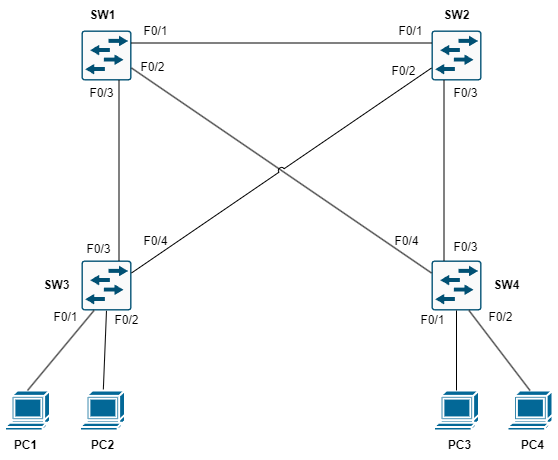
\includegraphics[width=0.8\textwidth]{img/rstp.png}
	\caption{\textit{}}
\end{figure}


\begin{enumerate}
	\item \textbf{Enable VTP and Set Server Mode on SW1 and VTP Client Mode on SW2, SW3, and SW4}
	      \begin{itemize}
		      \item Set the \textbf{VTP domain name} to \texttt{network} and the \textbf{password} to \texttt{network}.
		      \item Verify that all switches are using the same VTP domain and password.
	      \end{itemize}

	      %---,,,,,,,,,,,,,,,,,,,,,,,,,,,,,,,,,,---
	      \switchocg{codeblock}{%
		      \color{black}\underline{Click here to display the answer:}%
	      }


	      \begin{ocg}{Code Block}{codeblock}{0}
		      \vspace{0.5cm}
		      Server Mode on SW1:
		      \begin{lstlisting}
conf t
vtp mode server
vtp version 2
vtp domain network
vtp password network
end
    \end{lstlisting}



		      Client Mode on SW2, SW3, SW4:
		      \begin{lstlisting}
conf t
vtp mode client
vtp version 2
vtp domain network
vtp password network
end
\end{lstlisting}
	      \end{ocg}


	\item \textbf{Verify VTP Configuration}

	      %---,,,,,,,,,,,,,,,,,,,,,,,,,,,,,,,,,,---
	      \switchocg{codeblock}{%
		      \color{black}\underline{Click here to display the answer:}%
	      }


	      \begin{ocg}{Code Block}{codeblock}{0}
		      \vspace{0.5cm}
		      On all switches:
		      \begin{lstlisting}
show vtp status
        \end{lstlisting}
	      \end{ocg}
	      %---''''''''''''''''''''''''''''''''---

	      \vspace{1cm}

	      Since SW1 is the VTP Server, VLANs must be created here, and they will propagate to SW2, SW3, and SW4.
	\item \textbf{Create VLANs 1-30 on SW1}

	      %---,,,,,,,,,,,,,,,,,,,,,,,,,,,,,,,,,,---
	      \switchocg{codeblock}{%
		      \color{black}\underline{Click here to display the answer:}%
	      }


	      \begin{ocg}{Code Block}{codeblock}{0}
		      \vspace{0.5cm}

		      \begin{lstlisting}
conf t
vlan 1-30
exit
end
\end{lstlisting}
	      \end{ocg}
	      %---''''''''''''''''''''''''''''''''---
	\item \textbf{Verify VLAN Propagation}

	      %---,,,,,,,,,,,,,,,,,,,,,,,,,,,,,,,,,,---
	      \switchocg{codeblock}{%
		      \color{black}\underline{Click here to display the answer:}%
	      }


	      \begin{ocg}{Code Block}{codeblock}{0}
		      \vspace{0.5cm}
		      On SW2, SW3, and SW4:
		      \begin{lstlisting}
show vlan brief
\end{lstlisting}
	      \end{ocg}
	      %---''''''''''''''''''''''''''''''''---

	      \begin{itemize}
		      \item Ensure VLANs 1-30 are listed on all switches.
	      \end{itemize}
	      \vspace{1cm}

	      We now configure Multiple Spanning Tree (MST) on all switches.
	\item \textbf{Change the Spanning Tree Mode to MST}

	      %---,,,,,,,,,,,,,,,,,,,,,,,,,,,,,,,,,,---
	      \switchocg{codeblock}{%
		      \color{black}\underline{Click here to display the answer:}%
	      }


	      \begin{ocg}{Code Block}{codeblock}{0}
		      \vspace{0.5cm}
		      \begin{lstlisting}
 conf t
 spanning-tree mode mst
 end
 
 \end{lstlisting}
	      \end{ocg}
	      %---''''''''''''''''''''''''''''''''---


	\item \textbf{Verify MST Mode is Enabled}
	\item
	      %---,,,,,,,,,,,,,,,,,,,,,,,,,,,,,,,,,,---
	      \switchocg{codeblock}{%
		      \color{black}\underline{Click here to display the answer:}%
	      }


	      \begin{ocg}{Code Block}{codeblock}{0}
		      \vspace{0.5cm}
		      \begin{lstlisting}
show spanning-tree summary
\end{lstlisting}
	      \end{ocg}
	      %---''''''''''''''''''''''''''''''''---
	      \vspace{1cm}

	      The MST region name must match across all switches for them to share the same MST configuration.



	\item \textbf{Set MST Name and Revision Number on All Switches}


	      %---,,,,,,,,,,,,,,,,,,,,,,,,,,,,,,,,,,---
	      \switchocg{codeblock}{%
		      \color{black}\underline{Click here to display the answer:}%
	      }


	      \begin{ocg}{Code Block}{codeblock}{0}
		      \vspace{0.5cm}
		      \begin{lstlisting}
conf t
spanning-tree mst configuration
name network
revision 1
exit
end

\end{lstlisting}
	      \end{ocg}
	      %---''''''''''''''''''''''''''''''''---

	\item \textbf{Verify MST Configuration}

	      %---,,,,,,,,,,,,,,,,,,,,,,,,,,,,,,,,,,---
	      \switchocg{codeblock}{%
		      \color{black}\underline{Click here to display the answer:}%
	      }


	      \begin{ocg}{Code Block}{codeblock}{0}
		      \vspace{0.5cm}
		      \begin{lstlisting}
 show spanning-tree mst configuration
 \end{lstlisting}
	      \end{ocg}
	      %---''''''''''''''''''''''''''''''''---


	      \begin{itemize}
		      \item Ensure MST Name = network and Revision Number = 1 on all switches.
	      \end{itemize}
	      \vspace{1cm}
	      We now assign VLANs to different MST Instances.

	\item \textbf{Configure VLAN-to-Instance Mapping on All Switches}

	      %---,,,,,,,,,,,,,,,,,,,,,,,,,,,,,,,,,,---
	      \switchocg{codeblock}{%
		      \color{black}\underline{Click here to display the answer:}%
	      }


	      \begin{ocg}{Code Block}{codeblock}{0}
		      \vspace{0.5cm}
		      \begin{lstlisting}
conf t
spanning-tree mst configuration
instance 1 vlan 1-10
instance 2 vlan 11-20
instance 3 vlan 21-30
exit
end
\end{lstlisting}
	      \end{ocg}
	      %---''''''''''''''''''''''''''''''''---





	\item \textbf{Verify MST Instance Mapping}


	      %---,,,,,,,,,,,,,,,,,,,,,,,,,,,,,,,,,,---
	      \switchocg{codeblock}{%
		      \color{black}\underline{Click here to display the answer:}%
	      }


	      \begin{ocg}{Code Block}{codeblock}{0}
		      \vspace{0.5cm}
		      \begin{lstlisting}
show spanning-tree mst
\end{lstlisting}
	      \end{ocg}
	      %---''''''''''''''''''''''''''''''''---


	      \begin{itemize}
		      \item VLANs should be correctly mapped to their respective MST instances.
	      \end{itemize}

          \vspace{1cm}

          Now, we configure the Root Bridge per MST Instance.

	\item \textbf{Set SW1 as Root Bridge for MST Instance 1}
	

    %---,,,,,,,,,,,,,,,,,,,,,,,,,,,,,,,,,,---
    \switchocg{codeblock}{%
    \color{black}\underline{Click here to display the answer:}%
}


\begin{ocg}{Code Block}{codeblock}{0}
    \vspace{0.5cm}
    \begin{lstlisting}
conf t
spanning-tree mst 1 priority 4096
end
\end{lstlisting}
\end{ocg}
%---''''''''''''''''''''''''''''''''---


	\item \textbf{Set SW2 as Root Bridge for MST Instance 2}
	
    %---,,,,,,,,,,,,,,,,,,,,,,,,,,,,,,,,,,---
    \switchocg{codeblock}{%
    \color{black}\underline{Click here to display the answer:}%
}


\begin{ocg}{Code Block}{codeblock}{0}
    \vspace{0.5cm}
    \begin{lstlisting}
conf t
spanning-tree mst 2 priority 4096
end
\end{lstlisting}
\end{ocg}
%---''''''''''''''''''''''''''''''''---


	
	\item \textbf{Set SW3 as Root Bridge for MST Instance 3}
	
	%---,,,,,,,,,,,,,,,,,,,,,,,,,,,,,,,,,,---
    \switchocg{codeblock}{%
    \color{black}\underline{Click here to display the answer:}%
}


\begin{ocg}{Code Block}{codeblock}{0}
    \vspace{0.5cm}
    \begin{lstlisting}
conf t
spanning-tree mst 3 priority 4096
end
\end{lstlisting}
\end{ocg}
%---''''''''''''''''''''''''''''''''---


	\item \textbf{Verify Root Bridge Assignment}
    
    %---,,,,,,,,,,,,,,,,,,,,,,,,,,,,,,,,,,---
    \switchocg{codeblock}{%
    \color{black}\underline{Click here to display the answer:}%
}


\begin{ocg}{Code Block}{codeblock}{0}
    \vspace{0.5cm}
    \begin{lstlisting}
show spanning-tree mst
\end{lstlisting}
\end{ocg}
%---''''''''''''''''''''''''''''''''---


\begin{itemize}
    \item SW1 should be the Root for MST Instance 1.
    \item SW2 should be the Root for MST Instance 2.
    \item SW3 should be the Root for MST Instance 3.
\end{itemize}




	\item \textbf{Verify MST Configuration}
	
	%---,,,,,,,,,,,,,,,,,,,,,,,,,,,,,,,,,,---
    \switchocg{codeblock}{%
    \color{black}\underline{Click here to display the answer:}%
}


\begin{ocg}{Code Block}{codeblock}{0}
    \vspace{0.5cm}
    On each switch, run:
    \begin{lstlisting}
show spanning-tree mst configuration
show spanning-tree mst
show spanning-tree summary
\end{lstlisting}
\end{ocg}
%---''''''''''''''''''''''''''''''''---

\begin{itemize}
    \item Ensure VLAN mappings are correct.
    \item Verify Root Bridges for each MST Instance.
    \item Confirm all switches belong to the same MST Region.
\end{itemize}


\end{enumerate}


\end{document}